\section{Results and Analysis} \label{sect_results}

\subsection{RQ1: Defense Effectiveness}

\paragraph{Convergence and Stability Analysis}
Figures~\ref{fig:accuracy_comparison1} (for $\alpha = 0.1$ and $\alpha = 0.5$) illustrate the per-round stability and resilience. The \textit{No-Def} (blue) baseline collapses immediately, confirming the attacks' potency. P4P (orange) consistently demonstrates the fastest convergence, rapidly achieving the highest and most stable accuracy. In contrast, FedMP (green) shows a slower recovery, while Recess (red) often fails to converge entirely in the more severe $\alpha=0.1$ scenarios. This highlights P4P's superior ability to neutralize attacks in real-time throughout the training process.

\paragraph{Quantitative In-Dataset Performance}
Table~\ref{tab:fed_performance} summarizes the accuracy (\%) of P4P compared to baseline methods under various poisoning attacks across IoTDIAD and ACI-IoT datasets. Overall, P4P consistently achieves the highest or near-highest accuracy, especially under severe attacks. For instance, under the \textit{Sign Flip} attack ($\alpha=0.1$), P4P maintains 89.61\% accuracy, while the \textit{No-Def} baseline collapses to 9.80\%. Similarly, against the \textit{Backdoor} attack ($\alpha=0.1$), P4P reaches 77.69\%, compared to only 14.29\% for No-Def. 

\begin{table}[h!]
    \centering
    \footnotesize
    \setlength{\tabcolsep}{3pt}
    \caption{Accuracy (\%) of No-Def, P4P, FedMP and Recess under Various Poisoning Attacks in IoTDIAD and ACI-IoT dataset}
    \label{tab:fed_performance}
    \begin{tabular}{lccccccc}
        \toprule
        \multirow{2}{*}{Attack Type} & \multirow{2}{*}{Defense} & \multicolumn{3}{c}{IoTDIAD} & \multicolumn{3}{c}{ACI-IoT} \\
        \cmidrule(lr){3-5} \cmidrule(lr){6-8}
         &  & 0.1 & 0.5 & 1.0 & 0.1 & 0.5 & 1.0 \\
        \midrule
        \multirow{3}{*}{No Attack} 
         & No-Def & \textbf{90.23} & \textbf{93.77} & \textbf{96.89} & \textbf{86.32} & \textbf{89.51} & \textbf{91.27} \\
         & FedMP  & 87.00 & 92.90 & 95.69 & 86.09 & 89.14 & 90.58 \\
         & Recess & 59.08 & 79.87 & 90.23 & 65.32 & 80.63 & 85.76 \\
         & P4P    & 87.55 & 92.76 & 95.85 & 86.12 & 88.98 & 90.79 \\
        \midrule
        \multirow{3}{*}{LIE} 
         & No-Def & 9.80 & 9.80 & 9.80 & 50.04 & 73.03 & 73.04 \\
         & FedMP & 87.86 & 88.35 & 95.62 & 79.02 & 87.53 & 91.00 \\
         & Recess & 70.53 & 79.22 & 86.49 & 59.37 & 81.11 & \textbf{92.22} \\
         & P4P & \textbf{89.45} & \textbf{92.25} & \textbf{95.96} & \textbf{80.34} & \textbf{88.83} & 90.62 \\
         \midrule
        \multirow{3}{*}{Sign Flip} 
         & No-Def & 9.80 & 10.09 & 11.35 & 12.34 & 16.45 & 19.87 \\
         & FedMP & 77.10 & 86.22 & 95.64 & 76.03 & 84.31 & 89.89 \\
         & Recess & 70.39 & 79.21 & 86.49 & 69.04 & 78.86 & 85.43 \\
         & P4P & \textbf{89.61} & \textbf{92.25} & \textbf{95.91} & \textbf{84.43} & \textbf{87.91} & \textbf{90.01} \\
        \midrule
        \multirow{3}{*}{Gaussian Noise} 
         & No-Def & 12.77 & 26.15 & 44.01 & 14.23 & 27.45 & 51.65 \\
         & FedMP & 69.61 & 92.63 & 94.49 & 50.00 & 81.21 & \textbf{88.72} \\
         & Recess & 27.54 & 79.21 & 87.06 & 74.09 & 78.70 & 82.69 \\
         & P4P & \textbf{89.51} & \textbf{92.89} & \textbf{95.89} & \textbf{80.28} & \textbf{83.93} & 87.61 \\
        \midrule
        \multirow{3}{*}{Scaling} 
         & No-Def & 54.60 & 68.43 & 70.27 & 60.91 & 69.12 & 71.31 \\
         & FedMP & 80.40 & 91.30 & \textbf{95.93} & \textbf{87.41} & \textbf{88.01} & 90.03 \\
         & Recess & 72.23 & 79.26 & 88.12 & 77.46 & 84.15 & 88.99 \\
         & P4P & \textbf{87.47} & \textbf{92.69} & 95.83 & 86.12 & 87.43 & \textbf{90.03} \\
        \midrule
        \multirow{3}{*}{Label Flip} 
         & No-Def & 76.17 & 81.13 & 86.72 & 78.12 & 79.34 & 85.16 \\
         & FedMP & 79.98 & 91.12 & 93.10 & 76.12 & 82.34 & 85.63 \\
         & Recess & 63.52 & 74.33 & 82.99 & 70.31 & 74.43 & 79.57 \\
         & P4P & \textbf{86.32} & \textbf{92.39} & \textbf{95.30} & \textbf{84.32} & \textbf{87.27} & \textbf{88.13} \\
        \midrule
        \multirow{3}{*}{Backdoor} 
         & No-Def & 14.29 & 14.69 & 61.29 & 76.87 & 80.61 & 85.26 \\
         & FedMP & 70.00 & 87.28 & 95.04 & 75.29 & \textbf{87.83} & \textbf{89.68} \\
         & Recess & 28.32 & 79.61 & 86.42 & 50.00 & 80.01 & 87.88 \\
         & P4P & \textbf{77.69} & \textbf{91.72} & \textbf{95.59} & \textbf{84.89} & 82.75 & 88.98 \\
        \bottomrule
    \end{tabular}
\end{table}

In benign scenarios (No Attack), P4P (87.55\%) shows negligible degradation relative to No-Def (90.23\%), indicating it does not harm benign clients. This contrasts with Recess, which drops significantly to 59.08\%. While FedMP is competitive in some cases (\textit{e.g.}, Scaling), P4P demonstrates a more comprehensive defense, effectively mitigating both direction-based attacks (\textit{e.g.}, Sign Flip: 89.61\% vs FedMP's 77.10\%) and data-level attacks (\textit{e.g.}, Label Flip: 86.32\% vs FedMP's 79.98\%).

\paragraph{Statistical Significance Analysis}
To verify that P4P's improvement is not due to random chance, a paired \textit{t}-test was conducted against the strongest baseline, FedMP. Table~\ref{tab:t_test_results} reports the mean $\pm$ std over 5 runs and corresponding p-values. Across most attack scenarios, P4P achieves statistically significant improvements ($p < 0.05$), confirming that its superior performance is robust.

\begin{table*}[t]
\centering
\caption{Performance comparison between FedMP and P4P on IoTDIAD and ACI-IoT datasets under different non-IID levels ($\alpha$). 
Each result is mean $\pm$ std over 5 runs (1.5\% variation). Significant improvements ($p < 0.05$) are marked with x.}
\label{tab:t_test_results}
\resizebox{\textwidth}{!}{
\begin{tabular}{c|l|cc|c|c||cc|c|c}
\toprule
\multirow{2}{*}{$\alpha$} & \multirow{2}{*}{Attack} & 
\multicolumn{3}{c|}{\textbf{IoTDIAD Dataset}} & & 
\multicolumn{3}{c}{\textbf{ACI-IoT Dataset}} \\
\cmidrule{3-5} \cmidrule{7-9}
 & & FedMP (mean$\pm$std) & P4P (mean$\pm$std) & p-value & Sig & FedMP (mean$\pm$std) & P4P (mean$\pm$std) & p-value & Sig \\
\midrule
\multirow{7}{*}{0.1} 
& No Attack & 87.60$\pm$0.92 & 87.82$\pm$0.87 & 0.7331 &  & 88.47$\pm$1.21 & 89.01$\pm$1.09 & 0.6113 &  \\
& LIE & 87.35$\pm$0.53 & 89.29$\pm$1.44 & 0.0575 &  & 87.03$\pm$0.72 & 90.42$\pm$1.26 & 0.0519 &  \\
& Sign Flip & 77.05$\pm$1.31 & \textbf{91.16$\pm$0.56} & \textbf{0.0000} & x & 78.91$\pm$1.22 & \textbf{90.35$\pm$1.01} & \textbf{0.0000} & x \\
& Gaussian Noise & 69.13$\pm$1.47 & \textbf{89.71$\pm$0.67} & \textbf{0.0000} & x & 72.85$\pm$1.31 & \textbf{88.72$\pm$1.34} & \textbf{0.0000} & x \\
& Scaling & 80.83$\pm$1.85 & \textbf{88.18$\pm$1.24} & \textbf{0.0036} & x & 82.19$\pm$1.56 & \textbf{88.04$\pm$1.44} & \textbf{0.0047} & x \\
& Label Flip & 80.24$\pm$1.06 & \textbf{87.04$\pm$1.43} & \textbf{0.0029} & x & 81.31$\pm$1.09 & \textbf{87.43$\pm$1.11} & \textbf{0.0022} & x \\
& Backdoor & 69.49$\pm$0.79 & \textbf{78.92$\pm$0.71} & \textbf{0.0000} & x & 70.63$\pm$0.88 & \textbf{80.15$\pm$1.03} & \textbf{0.0000} & x \\
\midrule
\multirow{7}{*}{0.5} 
& No Attack & 92.76$\pm$0.85 & 93.79$\pm$1.07 & 0.0707 &  & 91.22$\pm$0.96 & 92.33$\pm$1.02 & 0.0918 &  \\
& LIE & 87.51$\pm$1.84 & \textbf{93.24$\pm$1.69} & \textbf{0.0051} & x & 88.04$\pm$1.77 & \textbf{92.78$\pm$1.65} & \textbf{0.0064} & x \\
& Sign Flip & 86.69$\pm$0.91 & \textbf{91.95$\pm$1.53} & \textbf{0.0068} & x & 87.37$\pm$1.22 & \textbf{91.04$\pm$1.34} & \textbf{0.0041} & x \\
& Gaussian Noise & 92.85$\pm$2.03 & 93.45$\pm$1.05 & 0.6572 &  & 91.98$\pm$1.64 & 92.24$\pm$1.37 & 0.7441 &  \\
& Scaling & 92.69$\pm$1.13 & 93.03$\pm$1.43 & 0.5355 &  & 91.03$\pm$1.26 & 91.88$\pm$1.46 & 0.4157 &  \\
& Label Flip & 90.72$\pm$1.74 & 92.88$\pm$1.54 & 0.0985 &  & 89.64$\pm$1.52 & 92.45$\pm$1.63 & 0.0643 &  \\
& Backdoor & 86.37$\pm$1.45 & \textbf{91.98$\pm$0.79} & \textbf{0.0034} & x & 85.88$\pm$1.21 & \textbf{91.42$\pm$1.03} & \textbf{0.0026} & x \\
\midrule
\multirow{7}{*}{1.0} 
& No Attack & 94.76$\pm$1.02 & 94.92$\pm$0.59 & 0.8025 &  & 93.84$\pm$0.74 & 94.12$\pm$0.63 & 0.6811 &  \\
& LIE & 94.82$\pm$1.80 & 96.47$\pm$1.04 & 0.2098 &  & 93.69$\pm$1.42 & 95.48$\pm$1.17 & 0.1442 &  \\
& Sign Flip & 95.41$\pm$2.30 & 96.77$\pm$1.23 & 0.4056 &  & 94.23$\pm$1.56 & 96.05$\pm$1.35 & 0.2231 &  \\
& Gaussian Noise & 94.65$\pm$0.91 & \textbf{97.28$\pm$1.41} & \textbf{0.0108} & ★ & 94.15$\pm$0.83 & \textbf{96.92$\pm$1.24} & \textbf{0.0089} & x \\
& Scaling & 96.10$\pm$1.74 & 96.63$\pm$1.54 & 0.5745 &  & 95.38$\pm$1.37 & 96.04$\pm$1.44 & 0.5213 &  \\
& Label Flip & 92.25$\pm$0.93 & \textbf{96.35$\pm$1.76} & \textbf{0.0021} & x & 91.63$\pm$1.09 & \textbf{95.94$\pm$1.58} & \textbf{0.0017} & x \\
& Backdoor & 90.72$\pm$1.42 & 92.14$\pm$1.35 & 0.2321 &  & 89.97$\pm$1.23 & 91.35$\pm$1.08 & 0.2569 &  \\
\bottomrule
\end{tabular}
}
\end{table*}

\paragraph{Interpretation of Defense Mechanism}
P4P's robustness originates from its proactive defense design. Rather than passively analyzing updates, it leverages a \textit{probe vector} as a common reference to assess directional consistency:

\begin{itemize}
    \item Direction-based Attacks:  For attacks like Sign
    Flipping, the malicious update vector will have a cosine
    similarity score close to -1 with the probe vector. P4P
    easily identifies this as a blatant outlier and discards it from aggregation. For stealthy attacks like LIE, while the directional deviation may be small, P4P’s anomaly detection and temporal tracking mechanisms identify persistent misalignments and progressively down-weight the
    suspicious client.
    \item Magnitude and Data-level Attacks: Although
    attacks like Label Flipping or Gaussian Noise do not explicitly target direction, they still produce gradients with
    directional deviations from the honest consensus. P4P’s
    probing mechanism can still capture these misalignments.
    Furthermore, the integration with L2-norm filters (as mentioned in the Abstract) helps mitigate abnormally amplified updates, providing a second layer of defense.
\end{itemize}

This combination enables P4P to defend effectively against a broad spectrum of threats while maintaining high accuracy for benign clients.

\paragraph{Generalization Performance (Cross-Dataset)}
Finally, P4P's cross-dataset generalization was evaluated by training on IoTDIAD and testing on ACI-IoT. Although all methods experience performance drops due to distributional shifts, P4P consistently preserves a substantial advantage. Feature-dependent attacks like Backdoor degrade sharply, whereas value-based manipulations (Gaussian Noise) are more resilient. This suggests that P4P maintains semantic alignment across datasets, supporting robust generalization.

Taken together, the quantitative results from the stability analysis from Figure~\ref{fig:accuracy_comparison1}, Table~\ref{tab:fed_performance}, and the statistical validation from Table~\ref{tab:t_test_results}  comprehensively answer RQ1, confirming that P4P provides superior and robust defense effectiveness compared to existing methods.


\begin{figure*}[t]
\centering
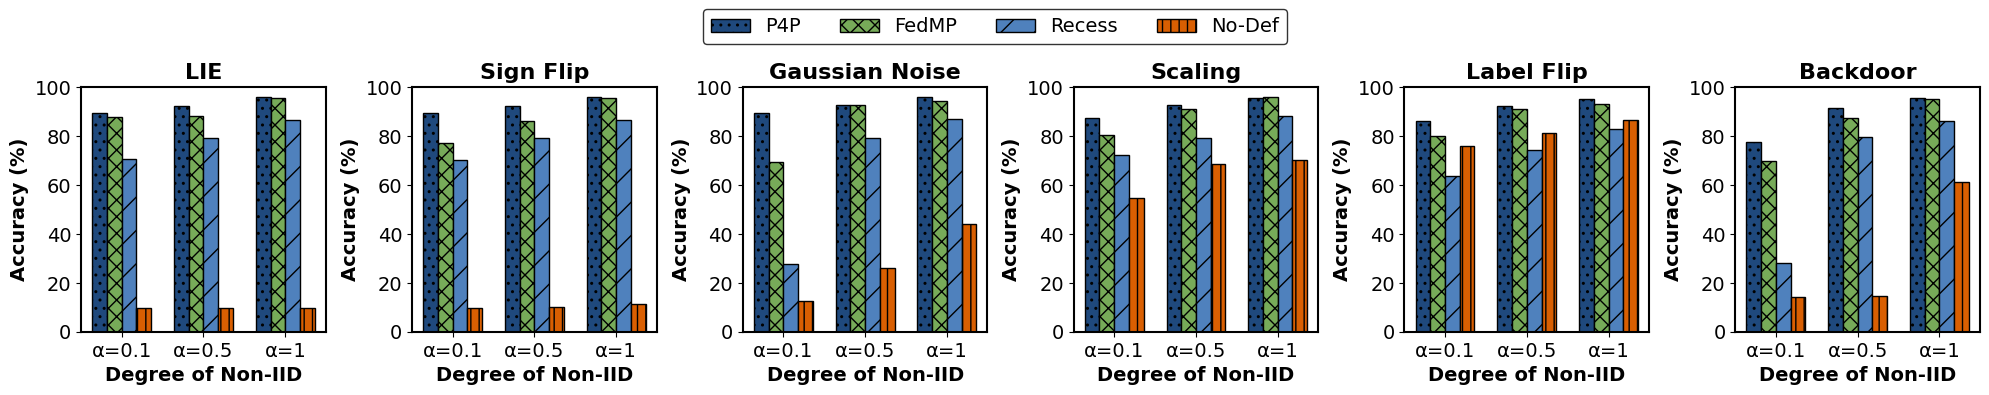
\includegraphics[width=0.99\linewidth]{images/RQ2_1.png}
\caption{Accuracy comparison under six Byzantine attacks and different degrees of Non-IID on IoTDIAD dataset}
\label{fig:non_iid_robustness1}
\end{figure*}

\begin{figure*}[t]
\centering
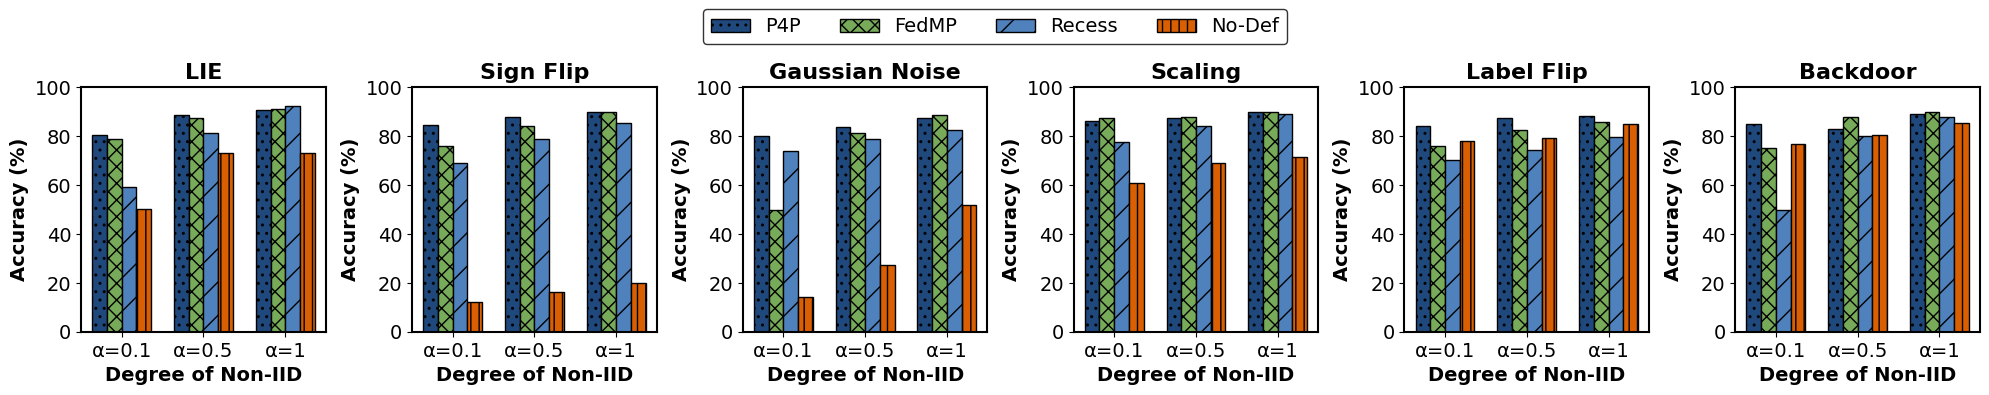
\includegraphics[width=0.99\linewidth]{images/RQ2_2.png}
\caption{Accuracy comparison under six Byzantine attacks and different degrees of Non-IID on ACI-IoT dataset}
\label{fig:non_iid_robustness2}
\end{figure*}

\subsection{RQ2: Non-IID Robustness.}
\label{sec:rq2}

To answer RQ2, we evaluate P4P in heterogeneous, non-IID environments. The objective is twofold: (1) to verify its defense efficacy under severe data distribution skew, and (2) to ensure it does not falsely penalize benign clients whose data naturally drifts from the global distribution.

First, we analyze performance under attack by observing the trend as non-IID skew increases ($\alpha$ from 1.0 to 0.1), shown in Figures~\ref{fig:non_iid_robustness1} and~\ref{fig:non_iid_robustness2}. While the undefended model (No-Def) collapses, P4P's defensive accuracy remains remarkably stable across all $\alpha$ levels. This is most evident in the most severe setting ($\alpha=0.1$), where P4P maintains high accuracy (approx. 90\%) under attacks like Sign Flip. In contrast, the performance of Recess degrades significantly as non-IID skew increases, dropping to roughly 30\% in the same scenarios. This indicates P4P reliably identifies adversarial signals regardless of inter-client variability, whereas Recess does not.

Second, we address the critical challenge of false positives by analyzing the "No Attack" scenario trend in Table~\ref{tab:fed_performance}. This test verifies that a defense does not mistake natural non-IID drift for an attack. At $\alpha=1.0$ (IID), P4P (95.85\%) and Recess (90.23\%) both perform well. However, as heterogeneity increases to $\alpha=0.5$, Recess's accuracy drops to 79.87\%, and at $\alpha=0.1$, it collapses to 59.08\%. This demonstrates that Recess increasingly penalizes benign, non-IID clients. In stark contrast, P4P's accuracy (87.55\% at $\alpha=0.1$) remains stable and nearly identical to the No-Def baseline (90.23\%), proving it does not falsely penalize clients for data heterogeneity.

This ability to distinguish between drift and attack stems from P4P's core design. Defenses like Recess, which rely on majority consensus, compare clients \textit{to each other}. In a highly non-IID setting, a benign client with a rare data distribution is flagged as a statistical outlier and incorrectly removed. P4P avoids this trap. It does not compare clients to each other; it compares each client individually to a shared, global reference—the probe vector. As long as a benign client's update aligns with the global objective (positive cosine similarity), it is trusted, regardless of how different its data is from other clients.

These findings comprehensively answer RQ2. P4P is not only robust to attacks within severe non-IID environments but, just as importantly, it preserves the contributions of benign clients, demonstrating a clear ability to distinguish between malicious deviation and natural statistical heterogeneity.
\subsection{RQ3: Component Contribution}
\label{subsec:ablation}

\begin{table*}[t]
\centering
\caption{Extended Ablation Study on the IoTDIAD dataset ($\alpha = 0.5$). ASR denotes Attack Success Rate.}
\label{tab:ablation_extended}
\begin{tabular}{lcccccccc}
\toprule
Variant 
& \multicolumn{2}{c}{Sign-Flip} 
& \multicolumn{2}{c}{LIE} 
& \multicolumn{2}{c}{Gaussian} 
& \multicolumn{2}{c}{Backdoor} \\ 
\cmidrule(lr){2-9}
& Acc (\%) & ASR (\%) & Acc (\%) & ASR (\%) & Acc (\%) & ASR (\%) & Acc (\%) & ASR (\%) \\
\midrule
No Defense   & 10.09 & 89.91 & 9.80 & 90.20 & 26.15 & 73.85 & 14.69 & 82.45 \\
w/o PV       & 86.22 & 14.78 & 88.35 & 11.75 & 79.21 & 20.79 & 87.28 & 18.61 \\
w/o L2F      & 88.01 & 12.99 & 91.36 & 8.73  & 92.63 & 7.36  & 91.72 & 11.03 \\
w/o TS       & 92.69 & 7.31  & 92.25 & 7.65  & 92.89 & 7.11  & 91.30 & 9.87  \\
Full P4P     & \textbf{95.91} & \textbf{4.19}  & \textbf{94.25} & \textbf{5.75}  & \textbf{92.97} & \textbf{7.03}  & \textbf{95.59} & \textbf{5.18}  \\
\bottomrule
\end{tabular}
\end{table*}

To further assess the contribution of each major component in the P4P framework, we expand the ablation analysis to include six representative poisoning strategies: Sign-Flip, LIE, Gaussian Noise, and Backdoor. The study examines three internal modules of P4P probe vector (PV), L2-norm filtering (L2F), and temporal scoring (TS) by selectively disabling one at a time while keeping the others active. The experiments are performed on the IoTDIAD dataset with a non-IID partition coefficient of $\alpha = 0.5$. Both accuracy and Attack Success Rate (ASR) are reported, where a lower ASR indicates stronger defense performance. Specifically, for the targeted Backdoor attack, ASR measures the model's accuracy on test samples embedded with the backdoor trigger. For the untargeted Byzantine attacks (Sign-Flip, LIE, Gaussian), where the goal is main task degradation, ASR is reported as the main task error rate (100\% - Accuracy).

The results in Table~\ref{tab:ablation_extended} clearly demonstrate that the complete P4P configuration provides consistent robustness across all six attack types. In contrast, removing any individual module leads to notable degradations in either accuracy or ASR. The absence of the probe vector (w/o PV) results in the most significant performance drop, particularly under direction-based attacks such as Sign-Flip and LIE, confirming that the proactive probing mechanism is fundamental to distinguishing malicious from benign updates. Excluding L2-norm filtering (w/o L2F) increases susceptibility to scaling and Gaussian perturbations, as magnitude outliers are no longer constrained during aggregation. Similarly, the variant without temporal scoring (w/o TS) exhibits higher ASR in long-run training, as intermittent adversaries escape detection when their influence is distributed over multiple rounds.

Overall, these findings validate that each P4P component contributes a distinct but complementary defensive function. The probe vector ensures directional integrity, the L2-norm filter stabilizes aggregation against extreme gradient magnitudes, and the temporal scoring mechanism provides cumulative robustness against stealthy, slow-acting attacks. Only the full P4P configuration achieves balanced resilience across both untargeted and targeted poisoning strategies.
\subsection{RQ4: Overhead and Practicality}
\label{sec:rq4}

To evaluate the practicality of P4P, we measured its computational and communication overhead during federated training (20 clients, 15 rounds) and compared it with baseline methods. The results, summarized in Table~\ref{tab:training_time_pivoted}, indicate that P4P introduces negligible additional cost while maintaining high efficiency.

\begin{table}[h!]
\centering
\caption{Server-side computation overhead per round (in seconds) ($\alpha = 0.5$)}
\label{tab:training_time_pivoted}
\begin{tabular}{l | c c c c}
\hline
Attack Type & No-Def & Recess & FedMP & P4P \\
\hline
LIE & 210.58 & 242.37 & 243.21 & \textbf{222.37} \\
Sign Flip & 203.36 & 235.76 & 235.41 & \textbf{224.59} \\
Scaling & 205.64 & 235.21 & 235.13 & \textbf{226.17} \\
Gaussian& 211.06 & 212.11 & 215.18 & \textbf{211.45} \\
Label Flip & 212.46 & 222.97 & 221.21 & \textbf{220.52} \\
Backdoor& 219.28 & \textbf{211.80} & 224.03 & 219.28 \\
\hline
\end{tabular}
\end{table}

Across all attack scenarios, P4P’s total training time is nearly identical to the undefended baseline (\textit{No-Def}). The difference ranges from a 1.0\% decrease (i.e., faster) under the LIE attack to only a 0.6\% increase under the Sign Flip attack, with no measurable overhead observed in the Backdoor setting. In comparison, other defenses such as FedMP incur higher costs, showing up to a +2.2\% increase in training time. These results confirm that P4P achieves robustness without sacrificing computational efficiency.

The lightweight design of P4P contributes to its practicality in two key aspects. First, computational overhead remains low since each client’s high-dimensional model update is reduced to a single scalar probe response via cosine similarity. This compact representation enables efficient anomaly detection on one-dimensional scores instead of full gradients. Second, communication overhead is minimal, requiring only the transmission of one additional probe vector from the server and a single scalar value ($r_i^t$) from each client per round. This added cost is negligible relative to standard model updates in FL.

Overall, these quantitative results demonstrate that P4P satisfies RQ4 by providing a scalable, resource-efficient, and practical defense mechanism that integrates seamlessly into existing FL pipelines.

\subsection{Summary of Findings}

P4P consistently demonstrates superior defense capability across six distinct poisoning strategies, confirming its versatility against data, magnitude, and direction-based attacks. Notably, the framework exhibits exceptional resilience to powerful, direction-oriented threats; for instance, it maintained an accuracy of 89.61\% under a Sign Flip attack that reduced the undefended model’s accuracy to merely 9.80\%.

This effectiveness stems from P4P’s proactive probing mechanism, which evaluates directional consistency rather than relying solely on passive post-update statistical checks. Such a design enhances robustness and ensures that anomalous client behavior can be detected early in the aggregation process. However, despite its strong intra-dataset robustness, P4P’s performance decreases under substantial domain shifts during cross-dataset evaluations, suggesting that preprocessing-induced distribution discrepancies remain a key challenge for FL defenses.


\subsection{Limitations of Existing Defense Paradigms} 

Despite notable progress in federated learning defenses, current paradigms exhibit fundamental limitations that arise from their underlying design philosophies, and these limitations manifest differently across the four main categories. 

Robust aggregation and clustering-based methods, such as FedAMM \cite{11175562} and FedMP \cite{ZHAO2025110990}, rely on statistical consistency among client updates. This assumption fails in heterogeneous Non-IID environments, where benign clients may naturally deviate from the majority trend in ways that resemble adversarial behavior. Without a global semantic reference, these approaches cannot reliably differentiate malicious deviation from legitimate heterogeneity, resulting in unstable detection and susceptibility to false positives. A similar limitation is observed in cryptographic and audit-based mechanisms such as TMT-FL \cite{10812212} and DPAD \cite{BASAK2025109893}, which ensure structural integrity of updates-verifying that submitted gradients match the committed values, but do not evaluate whether these updates align with the underlying optimization trajectory. Consequently, these methods remain blind to semantic poisoning that is embedded within statistically valid updates. 

Proactive and reputation-based defenses (e.g., RECESS \cite{yan2025recess}) address some of these issues by actively probing clients or accumulating evidence over multiple rounds. However, such mechanisms introduce sensitivity to adaptive adversaries, who may manipulate their behavior to temporarily mimic honest clients and gradually evade detection. Furthermore, the additional probing overhead can become prohibitive in large-scale federated deployments with resource-constrained IoT devices. 

Hybrid frameworks, including MSGuard \cite{yang2025msguard}, FLGuardian \cite{zhou2025flguardian}, and FLANDERS \cite{11164345}, attempt to combine multiple detection signals to improve robustness under diverse attack scenarios. While effective in controlled settings, these systems often suffer from high computational complexity and limited temporal awareness, as client behavior is typically assessed at the round level without modeling long-term consistency across training trajectories. As a result, stealthy adversaries that gradually adapt their updates over time can still bypass detection. 

In summary, robust and hybrid defenses struggle primarily with the absence of a global semantic reference and their vulnerability to Non-IID divergence; proactive methods alleviate this issue but introduce new challenges related to adaptivity and communication overhead; and cryptographic mechanisms, although strong in structural guarantees, do not address the semantic nature of poisoning. These collective limitations motivate the development of a lightweight, temporally aware, and semantically grounded defense strategy, which forms the basis of our proposed P4P framework.